\subsection{Kompleksitet}
\begin{frame}[fragile]{Kompleksitet}
    Gitt to algoritmer som løser det samme problemet, hvordan vite hvilken som er kjappest?
    %Vi kan kjøre begge to og ta tiden, men det hadde vært kjekt å vite svaret før vi bruker tid på å implementere noe som helst.
    \begin{columns}
        \begin{column}{0.45\textwidth}
            \begin{minted}[fontsize=\scriptsize]{python}
def minAndMax(list):
    min = list[0]
    for elem in list[1:]:
        if elem < min:
            min = elem
    max = list[0]
    for elem in list[1:]:
        if elem > max:
            max = elem
    return (min, max)
            \end{minted}
        \end{column}
        \pause
        \begin{column}{0.45\textwidth}
            \begin{minted}[fontsize=\scriptsize]{python}
def minAndMax(list):
    min, max = list[0], list[0]
    for elem in list[1:]:
        if elem < min: min = elem
        if elem > max: max = elem
    return (min, max)
    
def minAndMax(list):
    list = sorted(list)
    return (list[0], list[-1])
            \end{minted}
        \end{column}
    \end{columns}    
\end{frame}
\begin{frame}[fragile]{}
    Hvis vi hadde testet alle tre algoritmene på mange lister av økende lengde, ville det kanskje sett slik ut. Hvorfor?
    \begin{figure}
        \centering
        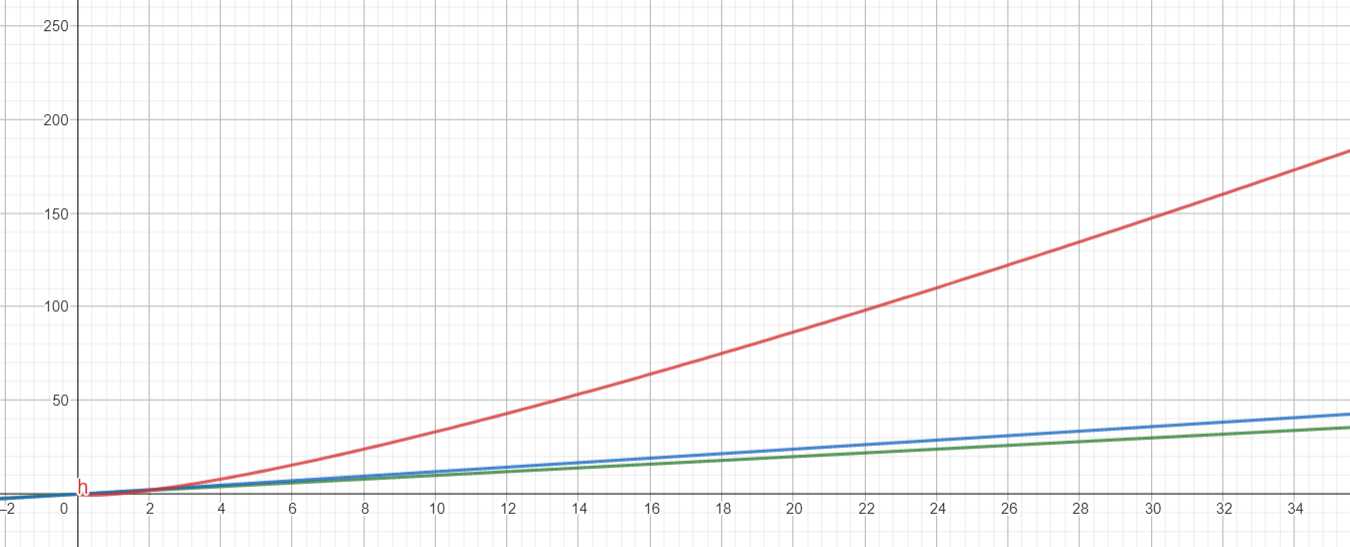
\includegraphics[height = 4.5cm]{images/minmax.png}
        \caption{Den røde er den som sorterer.}
        \label{fig:minmax}
    \end{figure}    
\end{frame}

\begin{frame}[fragile]{}
    La oss si at listen har en lengde på $n$. Hvor mange operasjoner blir det?
    \begin{columns}
        \begin{column}{0.45\textwidth}
            \begin{minted}[fontsize=\scriptsize]{python}
def minAndMax(list):
    min = list[0]         # 1
    for elem in list[1:]: # n-1
        if elem < min:    # 1
            min = elem    # 1
    max = list[0]         # 1
    for elem in list[1:]: # n-1
        if elem > max:    # 1
            max = elem    # 1
    return (min, max)
            \end{minted}
            Det blir ca $1 + (n-1)*(1+1) + 1 + (n-1)*(1+1) = 2 + 4*(n-1) = 4n-2$, og det er ihvertfall mindre enn \underline{$100n$}.
        \end{column}
        \pause
        \begin{column}{0.45\textwidth}
            \begin{minted}[fontsize=\scriptsize]{python}
def minAndMax(list):              
    min, max = list[0], list[0]   # 2
    for elem in list[1:]:         # n-1
        if elem < min: min = elem # 2
        if elem > max: max = elem # 2
    return (min, max)
    
def minAndMax(list):
    list = sorted(list)    # n * log2(n)
    return (list[0], list[-1]) # 2
            \end{minted}
            Den første blir $2+(n-1)*(2+2) = 2+4(n-1) = 4n-2$, som er mindre enn \underline{$100n$}.\\
            \pause
            Den andre blir $2 + n \cdot log_2(n)$, og det er mindre enn \underline{$100 \cdot n \cdot log_2(n)$}.
        \end{column}
    \end{columns}
\end{frame}

\begin{frame}{Big O}
    Nå skal vi formalisere konseptet om hvor godt noe skalerer.
    \begin{definition}[Big O]
        Gitt to funksjoner $f, g : \mathbb{N} \rightarrow \mathbb{N}$: \\
        Hvis $\exists c, n_0 : \forall n > n_0 : [ f(n) \leq c*g(n) ]$, da er $f = O(g)$.\\
        Intuitivt kan vi tenke at $f \leq g$.
    \end{definition}
    \pause
    I vårt eksempel fant vi at algoritmene bruker mindre enn $100n$, $100n$, og $100 \cdot n \cdot log_2(n)$ operasjoner, og da kjører algoritmene på $O(n)$, $O(n)$, og $O(n \cdot log(n))$.\\[2mm]
    Big O er en veldig kjapp og enkel måte å estimere hva slags forskjeller som betyr noe og ikke. Konstanter spiller nesten ingen rolle i det store bildet: $O(10n) = O(5n) = O(n)$.
\end{frame}

\begin{frame}[fragile]{Regneregler for Big O}
    Løkker gjør at innholdet blir gjort mange ganger, da ganger vi med innholdet.
    \begin{minted}[fontsize=\scriptsize]{python}
for _ in range(n):     # O(n)
    for _ in range(m): # O(m)
        do_something() # O(1)
# Total: O(n)*O(m)*O(1) = O(nm).
    \end{minted}
    \pause
    Om vi vil summere flere ting, tar vi det største. Om vi ikke vet hva som er størst beholder vi begge.  
    \begin{columns}
        \begin{column}{0.45\textwidth}
            \begin{minted}[fontsize=\scriptsize]{python}
    for _ in range(n): # O(n)
        do_something() # O(1)
    do_something()     # O(1)
    do_something()     # O(1)
    # Total: O(n) + O(1) + O(1) = O(n).  
            \end{minted}
        \end{column}
        \pause
        \begin{column}{0.45\textwidth}
            \begin{minted}[fontsize=\scriptsize]{python}
    for _ in range(n): # O(n)
        do_something() # O(1)
    for _ in range(m): # O(m)
        do_something() # O(1)
    # Total: O(n) + O(m) = O(n+m).
            \end{minted}
            
        \end{column}
    \end{columns}
\end{frame}